% !TEX root = ../vr_st.tex

\subsection{Spheres and their wedge sum}\label{ss:Sn}\label{sub:Sn and wedge sum}

For any integer $n \geq 1$ and real number $\rho > 0$, let $\bS^n(\rho)$ be the \defn{$n$-sphere} of radius $\rho$ centered at the origin of $\R^{n+1}$.
We consider it equipped with the geodesic distance and simplify notation writing \(\bS^n\) instead of \(\bS^n(1)\).
The constant 
\[\zeta_n = \arccos\Big(\frac{-1}{n+1}\Big)\] 
will play an important role.
It is the diameter of an inscribed regular $(n+1)$-simplex in $\bS^n$. 

\subsubsection{}\label{subsub:critical values of Sn}

\medskip\proposition
For any $m,n \in \N$ and linear cohomology operation $\theta$ we have:
\begin{enumerate}
	\item \(\crit(\bS^n) = \frac{1}{2}\zeta_n\),
	\item \(\firstdeath{m}{\bS^n} =
	\begin{cases}
		\frac{1}{2}\zeta_n & m = n, \\
		\hfil 0 & m \neq n,
	\end{cases}\)
	\item \(\firstdeath{\theta}{\bS^n} = 0\).
\end{enumerate}

\begin{proof}
	(1) Recall from \cite[Thm.~7.1]{lim2024vietoris} that for any $0 < r \leq \zeta_n$, the space $\VR_r(\bS^n)$ is homotopy equivalent to $\bS^n$, and the homotopy type of $\VR_r(\bS^n)$ changes at $\zeta_n$.
%	\footnote{
%		The case $n = 1$ has more information.
%		From \cite[Thm.~7.4]{adamaszek2017vietoris} it is known that $\VR_r(\bS^1)$ is homotopy equivalent to $\bS^{2n+1}$ for any $n \in \N$ and $\frac{2n\pi}{2n+1} < r \leq \frac{2(n+1)\pi}{2n+3}$.
%		For $d=1$ and $n > 1$ and one also has more information.
%		Recall that a metric space $(\cX, d)$ is said to be a \defn{geodesic space} if for each $x, y \in \cX$ there exists geodesic from $x$ to $y$ of length $d(x, y)$.
%		As stated in \cite[Prop.~7.10]{virk20201} one knows that if $\cX$ be a simply-connected geodesic space, then $\barc\rH_1(\cX) = \emptyset$.
%		Since the spheres we are considering are geodesic their $\rH_1$ barcode is empty.}
	This implies $\crit(\bS^n)=\frac{1}{2}\zeta_n$.

	(2) According to \cite{katz1983filling}, \(\fillrad(\bS^n) = \frac{1}{2}\zeta_n\).
	Applying \cref{ss:beta v.s. fillrad}, we obtain \(\firstdeath{n}{\bS^n} = \frac{1}{2}\zeta_n\).
    When $m\neq n$, the statement follows from the fact that the initial space in the filtration has a trivial degree $m$ reduced homology.

	(3) We apply a similar argument as in the $m\neq n$ case of (2). The statement follows from the fact that the initial space in the filtration has trivial $\img_\theta$.
\end{proof}

\subsubsection{}\label{ss:VRSn projection}

Let \(n \in \N\) and \(r \in (0, \zeta_n]\).
From the previous proposition we know that the spaces \(\VR_r(\bS^n)\) and \(\bS^n\) have the same homotopy type for any \(n \in \N\).
We now recall from \cite{adamaszek2020homotopy} a natural map realizing this equivalence.

We define the \defn{\(\VR_r(\bS^n)\)-projection}
\[
f_r^n \colon \VR_r(\bS^n) \to \R^{n+1} \setminus \set{0} \to \bS^n
\]
to be the composition of the map sending a formal linear combination $\sum\lambda_i x_i$ to the point \(\sum\lambda_i x_i\) in \(\bbR^{n+1}\) and the map sending a point in \(\R^{n+1} \setminus \set{0}\) to its radial projection.
Here and for the remainder of this work, we do not distinguish between a simplicial complex and its geometric realization.

The well-definedness of $f_r^n$ follows from a similar argument to that in \cite[Lemma 3]{lovasz1983self}.
While the original proof was carried out for Euclidean spheres, an analogous argument applies to geodesic spheres.

\medskip\proposition
The \(\VR_r(\bS^n)\)-projection is a homotopy equivalence when $r \in (0, \zeta_n]$.

\begin{proof}
    In \cite{adamaszek2018metric}, a new topology was introduced on the Vietoris--Rips complex, with which the authors proved that the $\VR_r(\bS^n)$-projection is a homotopy equivalence.
    More recently, \cite{gillespie2024vietoris} showed that the identity map is a weak equivalence between this new topology and the usual one.
    Consequently, the $\VR_r(\bS^n)$-projection is a weak equivalence for the usual Vietoris--Rips complex.
    By the Whitehead theorem, this weak equivalence between CW spaces is indeed a homotopy equivalence.
\end{proof}

\subsubsection{}

\label{subsub:barcode_Sn}

We apply \cref{subsub:critical values of Sn} and the barcode estimates from \cref{ss:barcode_general} to \(\bS^n\).
Using the facts that (1) the reduced homology of \(\bS^n\) has dimension one for \(m = n\) and is zero for all other values of \(m\), and (2) for any linear cohomology operation \(\theta \in \cO(\ell, m)\) with \(\ell \neq m\), \(\img \theta_{\bS^n}\) is trivial, we proceed with the estimation but omit the figure, as it is simply a special case of \cref{fig:barcodes_vs}.

\subsubsection{}
\label{ss:barcodes_VS}

For $n \in \N$ and $u_1, \dots, u_n \in \N^n$, let
\[
\VS^{u_1,\dots,u_n} =
\overbrace{\bS^1\vee\dots\vee\bS^1}^{u_1} \vee\dots\vee \overbrace{\bS^n\vee\dots\vee\bS^n}^{u_n}.
%(\bS^1)^{\vee m_1} \vee \dots \vee (\bS^n)^{\vee m_n}.
\]
Using the homotopy equivalence between the Vietoris--Rips complex of a metric gluing with the wedge sum of the Vietoris--Rips complex described in \cref{ss:wedge sum}, we have the following isomorphisms of persistence modules for \(\degp \in \N\) and \(\theta \in \cO(\ell,\degp)\):
\[
\begin{split}
	\rH_\degp^\VR(\VS^{u_1,\dots,u_n}) &\cong \, \bigoplus_{i=1}^n \rH_\degp^\VR(\bS^i)^{\oplus u_i}, \\
	\img_\theta^\VR(\VS^{u_1,\dots,u_n}) &\cong \, \bigoplus_{i=1}^n \img_\theta^\VR(\bS^i)^{\oplus u_i}.
\end{split}
\]

Therefore, both the homology barcodes and \(\img_\theta\)-barcodes of \(\VR(\VS^{u_1, \dots, u_n})\) are the multiset unions of the corresponding barcodes of \(\bS^{u_i}\); see \cref{fig:barcodes_vs}.

\begin{figure}
	\centering
	\begin{tikzpicture}[scale=0.52]
	\begin{axis} [
		title = {\LARGE $\Hbarc[\field]{\degp}{\VS^n},1\leq \degp\leq n$},
		ticklabel style = {font=\Large},
		axis y line=middle,
		axis x line=middle,
		ytick={0.5,0.6,0.67,0.95},
		yticklabels={,$\zeta_\degp$,,$\pi$},
		xtick={0.5,0.55,0.95},
		xticklabels={$\frac{\pi}{2}$,$\zeta_n$, $\pi$},
		xmin=-0.015, xmax=1.1,
		ymin=0, ymax=1.1,]
		\addplot [mark=none] coordinates {(0,0) (1,1)};
		\addplot [thick,color=black!20!white,fill=black!30!white,
		fill opacity=0.4]coordinates {
			(0.55,0.95)
			(0.55,0.55)
			(0.95,0.95)
			(0.55,0.95)};
		\addplot [black!40!white,mark=none,dashed, thin] coordinates {(0,0.6) (0.6,0.6)};
		\addplot [black!40!white,mark=none,dashed, thin] coordinates {(0,0.55) (0.55,0.55)};
		\addplot [black!40!white,mark=none,dashed, thin] coordinates {(0.55,0) (0.55,0.55)};
		\addplot[barccolor,mark=*] (0, 0.6) circle (2pt) node[above right,barccolor]{};%{\Large\textsf{1}};
		%\node[mark=none] at (axis cs:0.68,0.21){$\Hbarc{2}{\VS^n}$};
	\end{axis}
\end{tikzpicture}
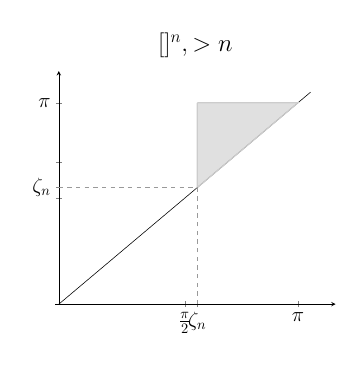
\begin{tikzpicture}[scale=0.52]
	\begin{axis} [
		title = {\LARGE $\Hbarc[\field]{\degp}{\VS^n}, \degp>n$},
		ticklabel style = {font=\Large},
		axis y line=middle,
		axis x line=middle,
		ytick={0.5,0.55,0.67,0.95},
		yticklabels={,$\zeta_n$,,$\pi$},
		xtick={0.5,0.55,0.95},
		xticklabels={$\frac{\pi}{2}$,$\zeta_n$, $\pi$},
		xmin=-0.015, xmax=1.1,
		ymin=0, ymax=1.1,]
		\addplot [mark=none] coordinates {(0,0) (1,1)};
		\addplot [thick,color=black!20!white,fill=black!30!white,
		fill opacity=0.4]coordinates {
			(0.55,0.95)
			(0.55,0.55)
			(0.95,0.95)
			(0.55,0.95)};
		\addplot [black!40!white,mark=none,dashed, thin] coordinates {(0,0.55) (0.55,0.55)};
		\addplot [black!40!white,mark=none,dashed, thin] coordinates {(0.55,0) (0.55,0.55)};
		%\node[mark=none] at (axis cs:0.68,0.21){$\Hbarc[\field]{\degp}{\VS^n}, \degp\geq 3$};
	\end{axis}
\end{tikzpicture}

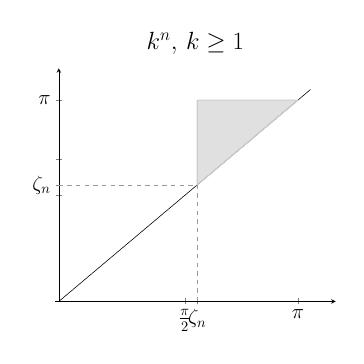
\begin{tikzpicture}[scale=0.52]
	\begin{axis} [
		title={\LARGE $\sqbarc{k}{\VS^n},\, k\geq 1$},
		ticklabel style = {font=\Large},
		axis y line=middle,
		axis x line=middle,
		ytick={0.5,0.55,0.67,0.95},
		yticklabels={,$\zeta_n$,,$\pi$},
		xtick={0.5,0.55,0.95},
		xticklabels={$\frac{\pi}{2}$,$\zeta_n$, $\pi$},
		xmin=-0.015, xmax=1.1,
		ymin=0, ymax=1.1,]
		\addplot [mark=none] coordinates {(0,0) (1,1)};
		\addplot [thick,color=black!20!white,fill=black!30!white,
		fill opacity=0.4]coordinates {
			(0.55,0.95)
			(0.55,0.55)
			(0.95,0.95)
			(0.55,0.95)};
		\addplot [black!40!white,mark=none,dashed, thin] coordinates {(0,0.55) (0.55,0.55)};
		\addplot [black!40!white,mark=none,dashed, thin] coordinates {(0.55,0) (0.55,0.55)};
		%\node[mark=none] at (axis cs:0.68,0.21){$\sqbarc{k}{\VS^n},\, k\geq 1$};
	\end{axis}
\end{tikzpicture}

	\caption{Let $\VS = \VS^{u_1,\dots,u_n}$ for some tuple of non-negative integers.
		\emph{Top row:} persistent reduced homology barcodes of $\VS$, where the dot $(0,\zeta_m)$ has multiplicity $u_m$ which can be zero.
		\emph{Bottom row:} $\img_\theta$-barcodes of $\VS$ where $\theta \in \cO(\ell,m)$ with \(\ell \neq m\).
        In each figure, the gray region represents where additional bars could exist within the corresponding barcode.
        See \cref{subsub:barcode_Sn} for the case when the wedge sum is a single sphere and see \cref{ss:barcodes_VS} for the general case.}
	\label{fig:barcodes_vs}
\end{figure}